\begin{figure*}[t]
\centering
\mpage{0.45}{
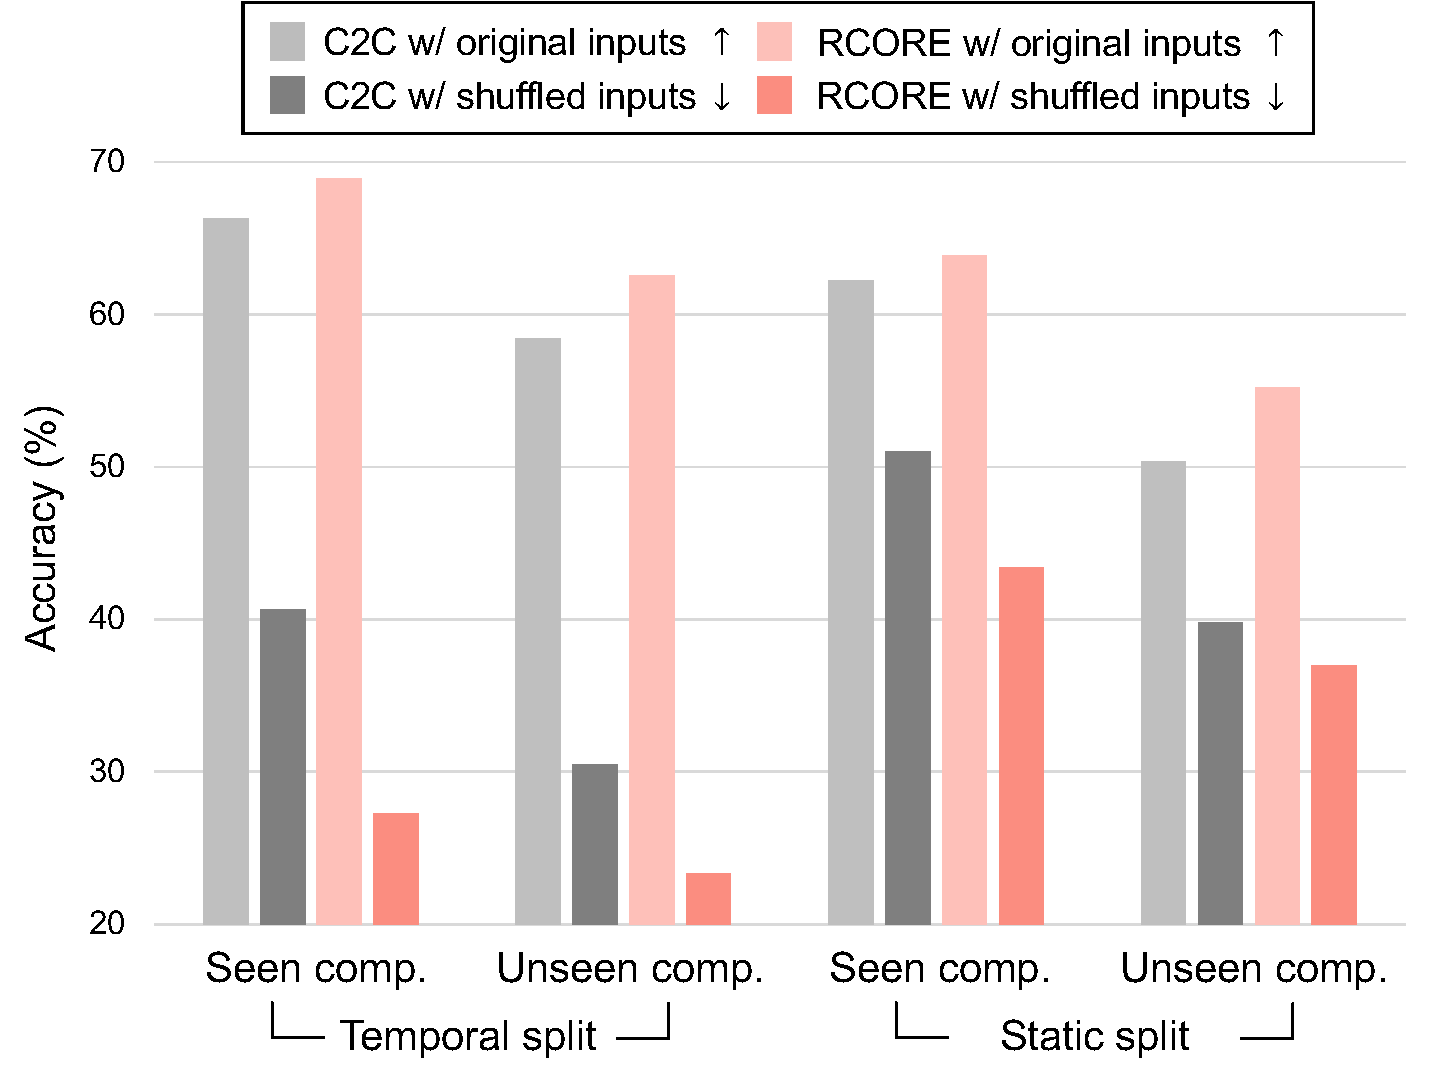
\includegraphics[width=\linewidth]{figure/supple_src/temporal_static_full_ver.pdf}}
\mpage{0.45}{
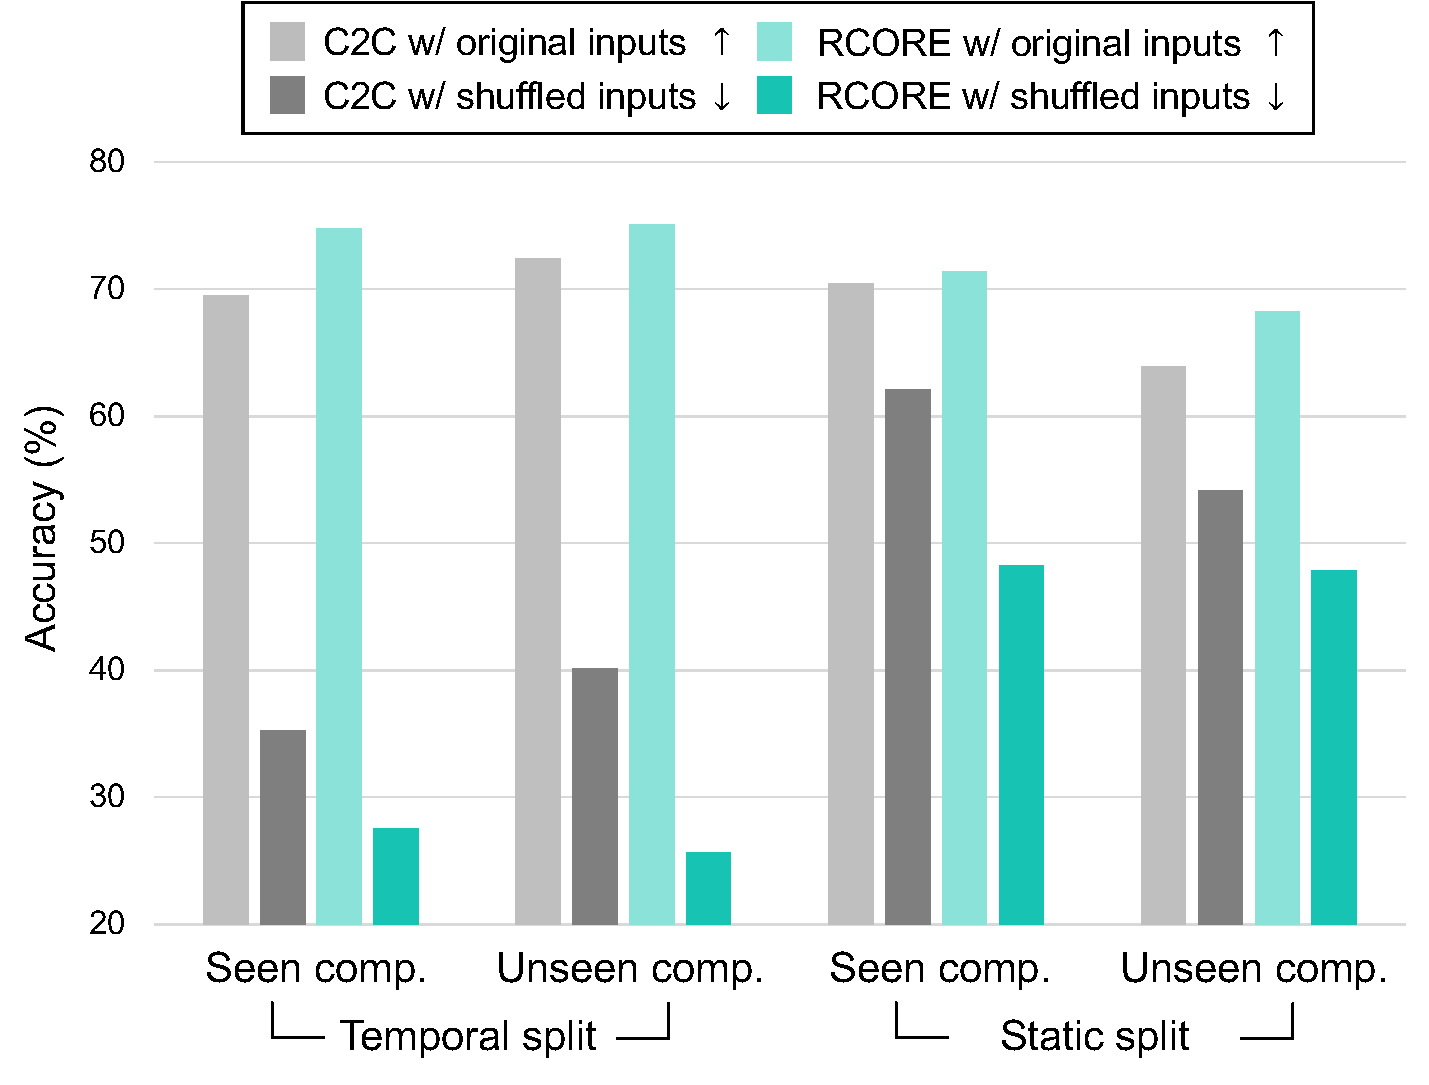
\includegraphics[width=\linewidth]{figure/supple_src/temporal_static_original_full_ver.pdf}}
\\
\mpage{0.45}{\scriptsize
(a) Our reconstructed Temporal/Static splits}
\mpage{0.45}{
\scriptsize (b) Temporal/Static splits from Sevilla et al.~\cite{laura2021temporal}}
\\
\figcapmargin
\figcaption{Performances on Temporal/Static split of Sth-com}{We evaluate the models on Sth-com~\cite{li2024c2c} using both (a) our reconstructed splits and (b) the splits from Sevilla et al~\cite{laura2021temporal}. 
We utilize both original and temporally shuffled inputs to assess the model’s temporal modeling capability and its reliance on static cues. 
A larger performance gap between original and shuffled inputs indicates that the model predicts verbs more based on temporal dynamics rather than on static cues.}
\label{fig:temporal_static_full}
\end{figure*}

